%/!\ ici on parle en terme d'architecture, donc ce qu'on a décidé AVANT d'implémenter


\section{L'architecture générale}

Nous avons choisi dès le départ de suivre une architecture de type MVC, et nous nous y sommes tenu tout au long du projet. Afin de nous faciliter le découpage du code et de définir nos principales interfaces, nous
avons conçu au démarrage du projet une architecture globale. Elle est représentée dans la figure \ref{Architecture}.

\begin{figure}[h!]
\centering
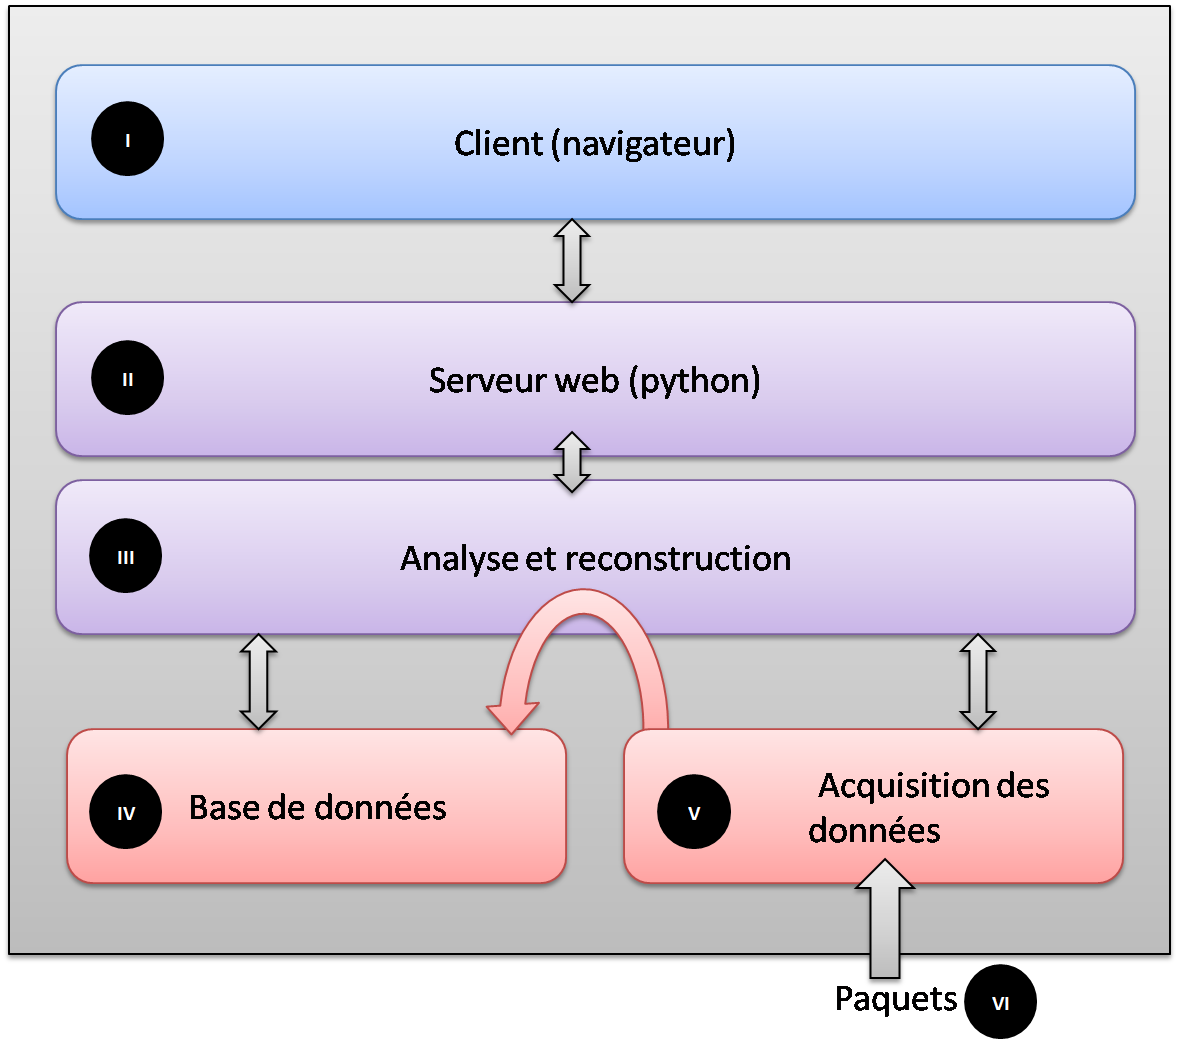
\includegraphics[scale=0.5]{Archi.png}
\caption{Architecture de Sniffeirb}
\label{Architecture}
\end{figure}

Nous avons choisi d'utiliser le langage Python pour notre projet, en partie pour ses nombreuses bibliothèques, y compris pour les captures réseaux. De plus, nous avions tous envie d'approfondir nos connaissances dans 
un langage de programmation autre que le C, C++ ou Java.

\section{Explication du rôle des différentes couches}

\subsection{Client}
Le client est soit le terminal dans lequel on lance le programme, soit un navigateur web. Nous n'offrons pas tout à fait les mêmes services sur ces deux interfaces, ceci est lié à notre volonté d'avoir une interface utilisateur simple. 
De ce fait, le terminal permet seulement de lancer une capture, ou de lancer le programme avec différentes options (lancement du serveur web, choix d'une ancienne capture à charger, choix du nom de la nouvelle capture, chargement d'un fichier pcap..).
L'interface web permet de lancer une capture, d'afficher les flux des différentes communications, de reconstruire les documents et de changer certains paramètres.

Le navigateur utilise des requêtes AJAX afin d'interagir avec  le programme.
Dans le but de fournir un programme utilisable sur le plus grand nombre de navigateur possible, nous avons utilisé des frameworks reconnus dans le milieu. Nous avons donc choisi d'utiliser JQuery pour nos requêtes, Bootstrap pour la mise en page et le CSS, et DataTables pour la présentation des flux sous forme de tableau. 

\subsection{Serveur web}
Le serveur web est l'interface entre les requêtes HTML provenant du client et les différentes actions possibles du sniffer. Après avoir lancé une action, le serveur renvoie si besoin est des données au navigateur au format
JSON. Nous n'avons pas utilisé de serveur déjà fourni dans un framework Python, trop lourd pour l'utilisation que nous en faisons.
Nous avons choisi d'utiliser JSON pour plusieurs raisons. C'est un format de données structuré, moins verbeux que le XML, et qui est très bien intégré avec le JavaScript et le Python. De plus le format JSON est identique au format BSON utilisé par la base de données. 

\subsection{Analyse et reconstruction}
Ce composant analyse une communication pour déterminer son protocole, reconstruit les flux possibles et reconstruit les documents qui transitent en donnant un pourcentage de validité. Nous assurons seulement la reconstruction des documents sur le protocle HTTP conformément à nos spécifications fonctionnelles.

\subsection{Base de données}
La base de données sert à stocker les paquets réseaux regroupés par communication. Stocker les données nous permet de rejouer des échanges de données (soit pour le débugage, soit suite à une amélioration algorithmique du projet).	
Nous avons choisi d'utiliser la base NoSQL Mongo pour ses performances et sa souplesse. Elle s'utilise aisément en Python grâce au module Pymongo. Il faut donc installer mongodb et lancer le service mongod pour pouvoir utiliser le sniffer.

\subsection{Acquisition des données}
Ce composant récupère les données réseaux, ou lit un fichier pcap, et les met dans la base de données. Les paquets sont regroupés par communication.
Nous utilisons le module Scapy de Python afin de récupérer les paquets. Il est de plus au même niveau que la bibliothèque Libpcap ou WinPcap, ce qui facilite la capture des paquets réseau. 

\subsection{Paquets}
Ceci représente le réseau, et les paquets qui circulent. En paramétrant la carte réseau en mode monitor, l'utilisateur peut alors écouter tout le réseau et analyser les paquets sniffés.


